\documentclass[dvipsnames, svgnames, x11names]{beamer}
\usetheme{mytheme}


\title{第五章}
\subtitle{电解质溶液}
\author{张斌}
\institute[理工系]{河北农业大学 理工系}
\date{\the\year 年 \the\month 月}

\begin{document}


	\begin{frame}
		\titlepage
		\thispagestyle{empty}
		\addtocounter{framenumber}{-1}
	\end{frame}


	\begin{frame}
		\frametitle{电解质溶液}
	
		电解质溶液(electrolyte solution)是离子导电体，依靠溶液中存在的离子迁移而导电，导电的同时在电极上发生化学反应。电解质溶液具有许多与一般物质溶液不同的特性。在本章中，我们将介绍        
		\begin{itemize}
			\item[\bullet] 离子的电迁移
			\item[\bullet] 电导、电导率和摩尔电导率等基本概念
			\item[\bullet] 电导测定的基本原理及应用
			\item[\bullet] 强电解质溶液导电特性与浓度的关系
			\item[\bullet] 离子独立运动定律
			\item[\bullet] 强电解质溶液的活度及活度系数
		\end{itemize}
	
	\end{frame}


	\begin{frame}{}
        \begin{center}
            {\Huge \cbf{目 \ 录}}
        \end{center}
		\tableofcontents
		\thispagestyle{empty}
		\addtocounter{framenumber}{-1}
	\end{frame}



	\section{离子的电迁移}


	\begin{frame}
		\frametitle{电解质溶液的导电机理}
		\begin{columns}[c]
			\column{8cm}
			能导电的物质称为导体。导体分为两类：
			\begin{enumerate}
			\item 电子导体，依靠自由电子的迁移导电；
			\item 离子导体，依靠离子的迁移导电。
			\end{enumerate}
			以电解\ch{CuCl2}水溶液为例。
			
			将两个铂电极连接外电源，并插入\ch{CuCl2}水溶液中，当有电流通过电解质溶液时，溶液中的\ch{Cu2+}在电场作用下向阴极(cathode)移动，\ch{Cl-}向阳极移动，当外加电势足够高时，\ch{Cu2+}与阴极上的电子相结合发生还原反应生成金属Cu，同时阳极上\ch{Cl-}给出电子发生氧化反应放出氯气。
			\column{5.5cm}
			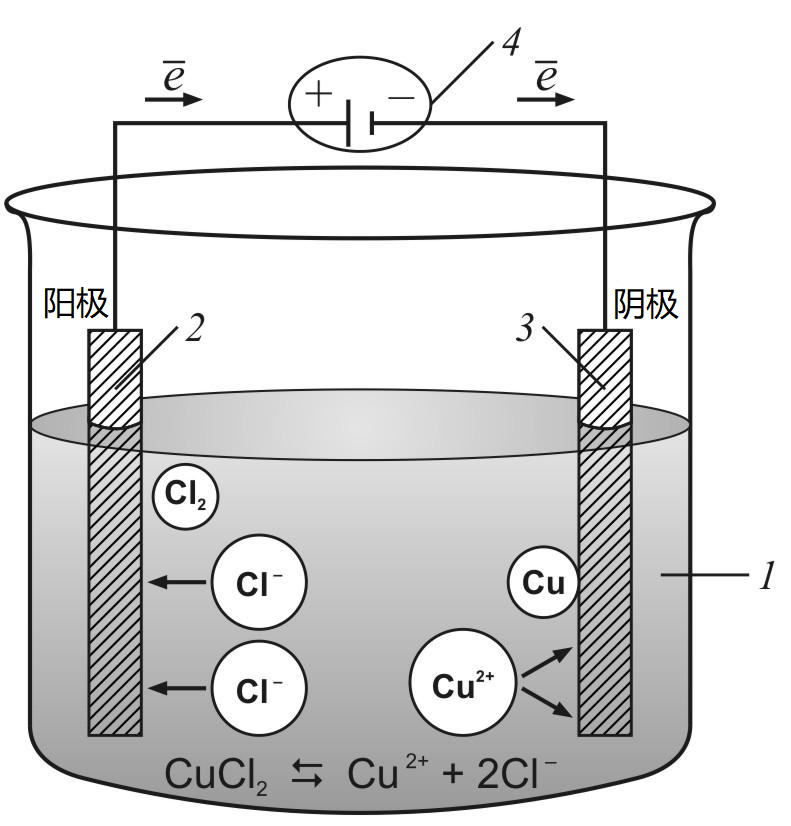
\includegraphics[width=5.2cm]{figs/fig5.0.png}
			\small 阳极 \ch{2 Cl- (aq) -> Cl2 (g) + 2 e-}
	
			阴极 \ch{Cu2+ (aq) + 2 e- -> Cu(s)}
	
			总 \ch{CuCl2 (aq) <=> Cu(s) + Cl2(g)}
		\end{columns}
	
	\end{frame}
	
	
	\begin{frame}
		\frametitle{电解池和原电池}
	
		\quad 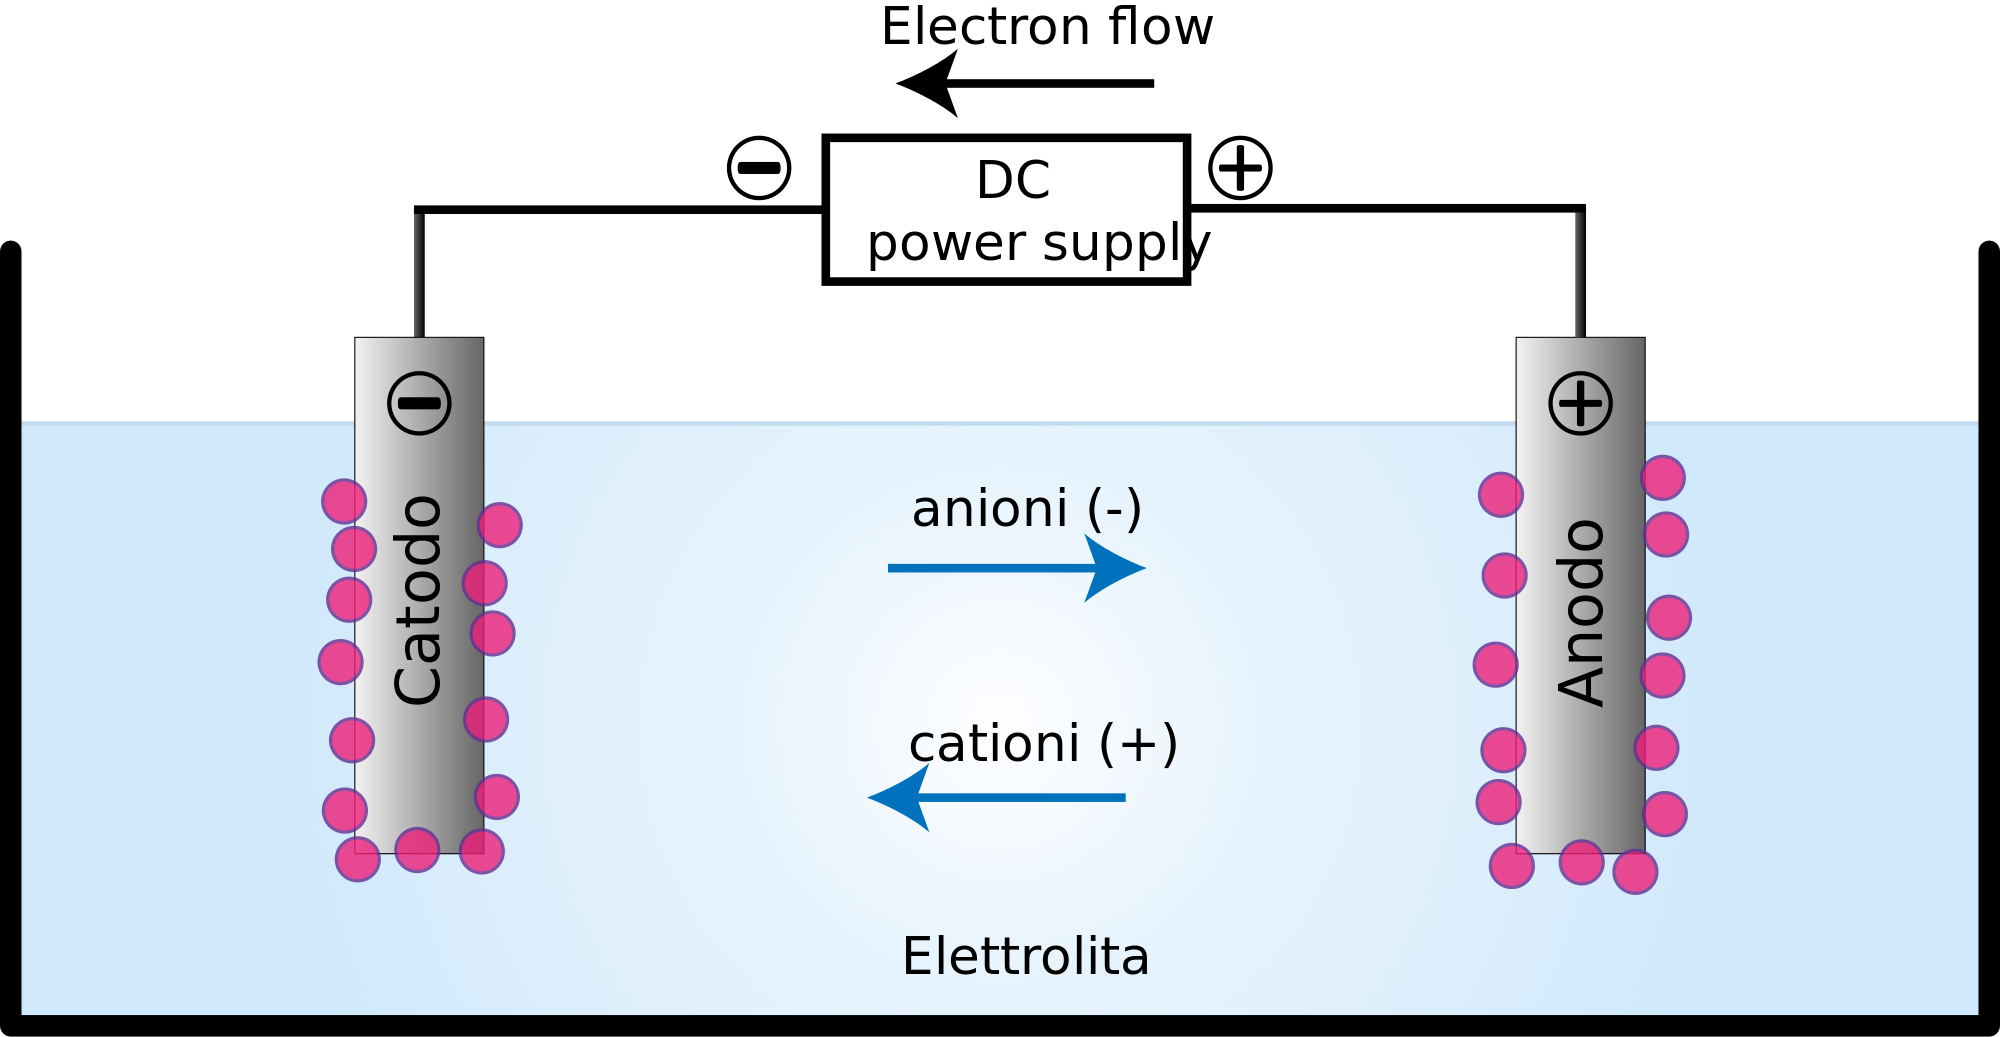
\includegraphics[width=.43\linewidth]{figs/electrolytic-cell.png} \qquad 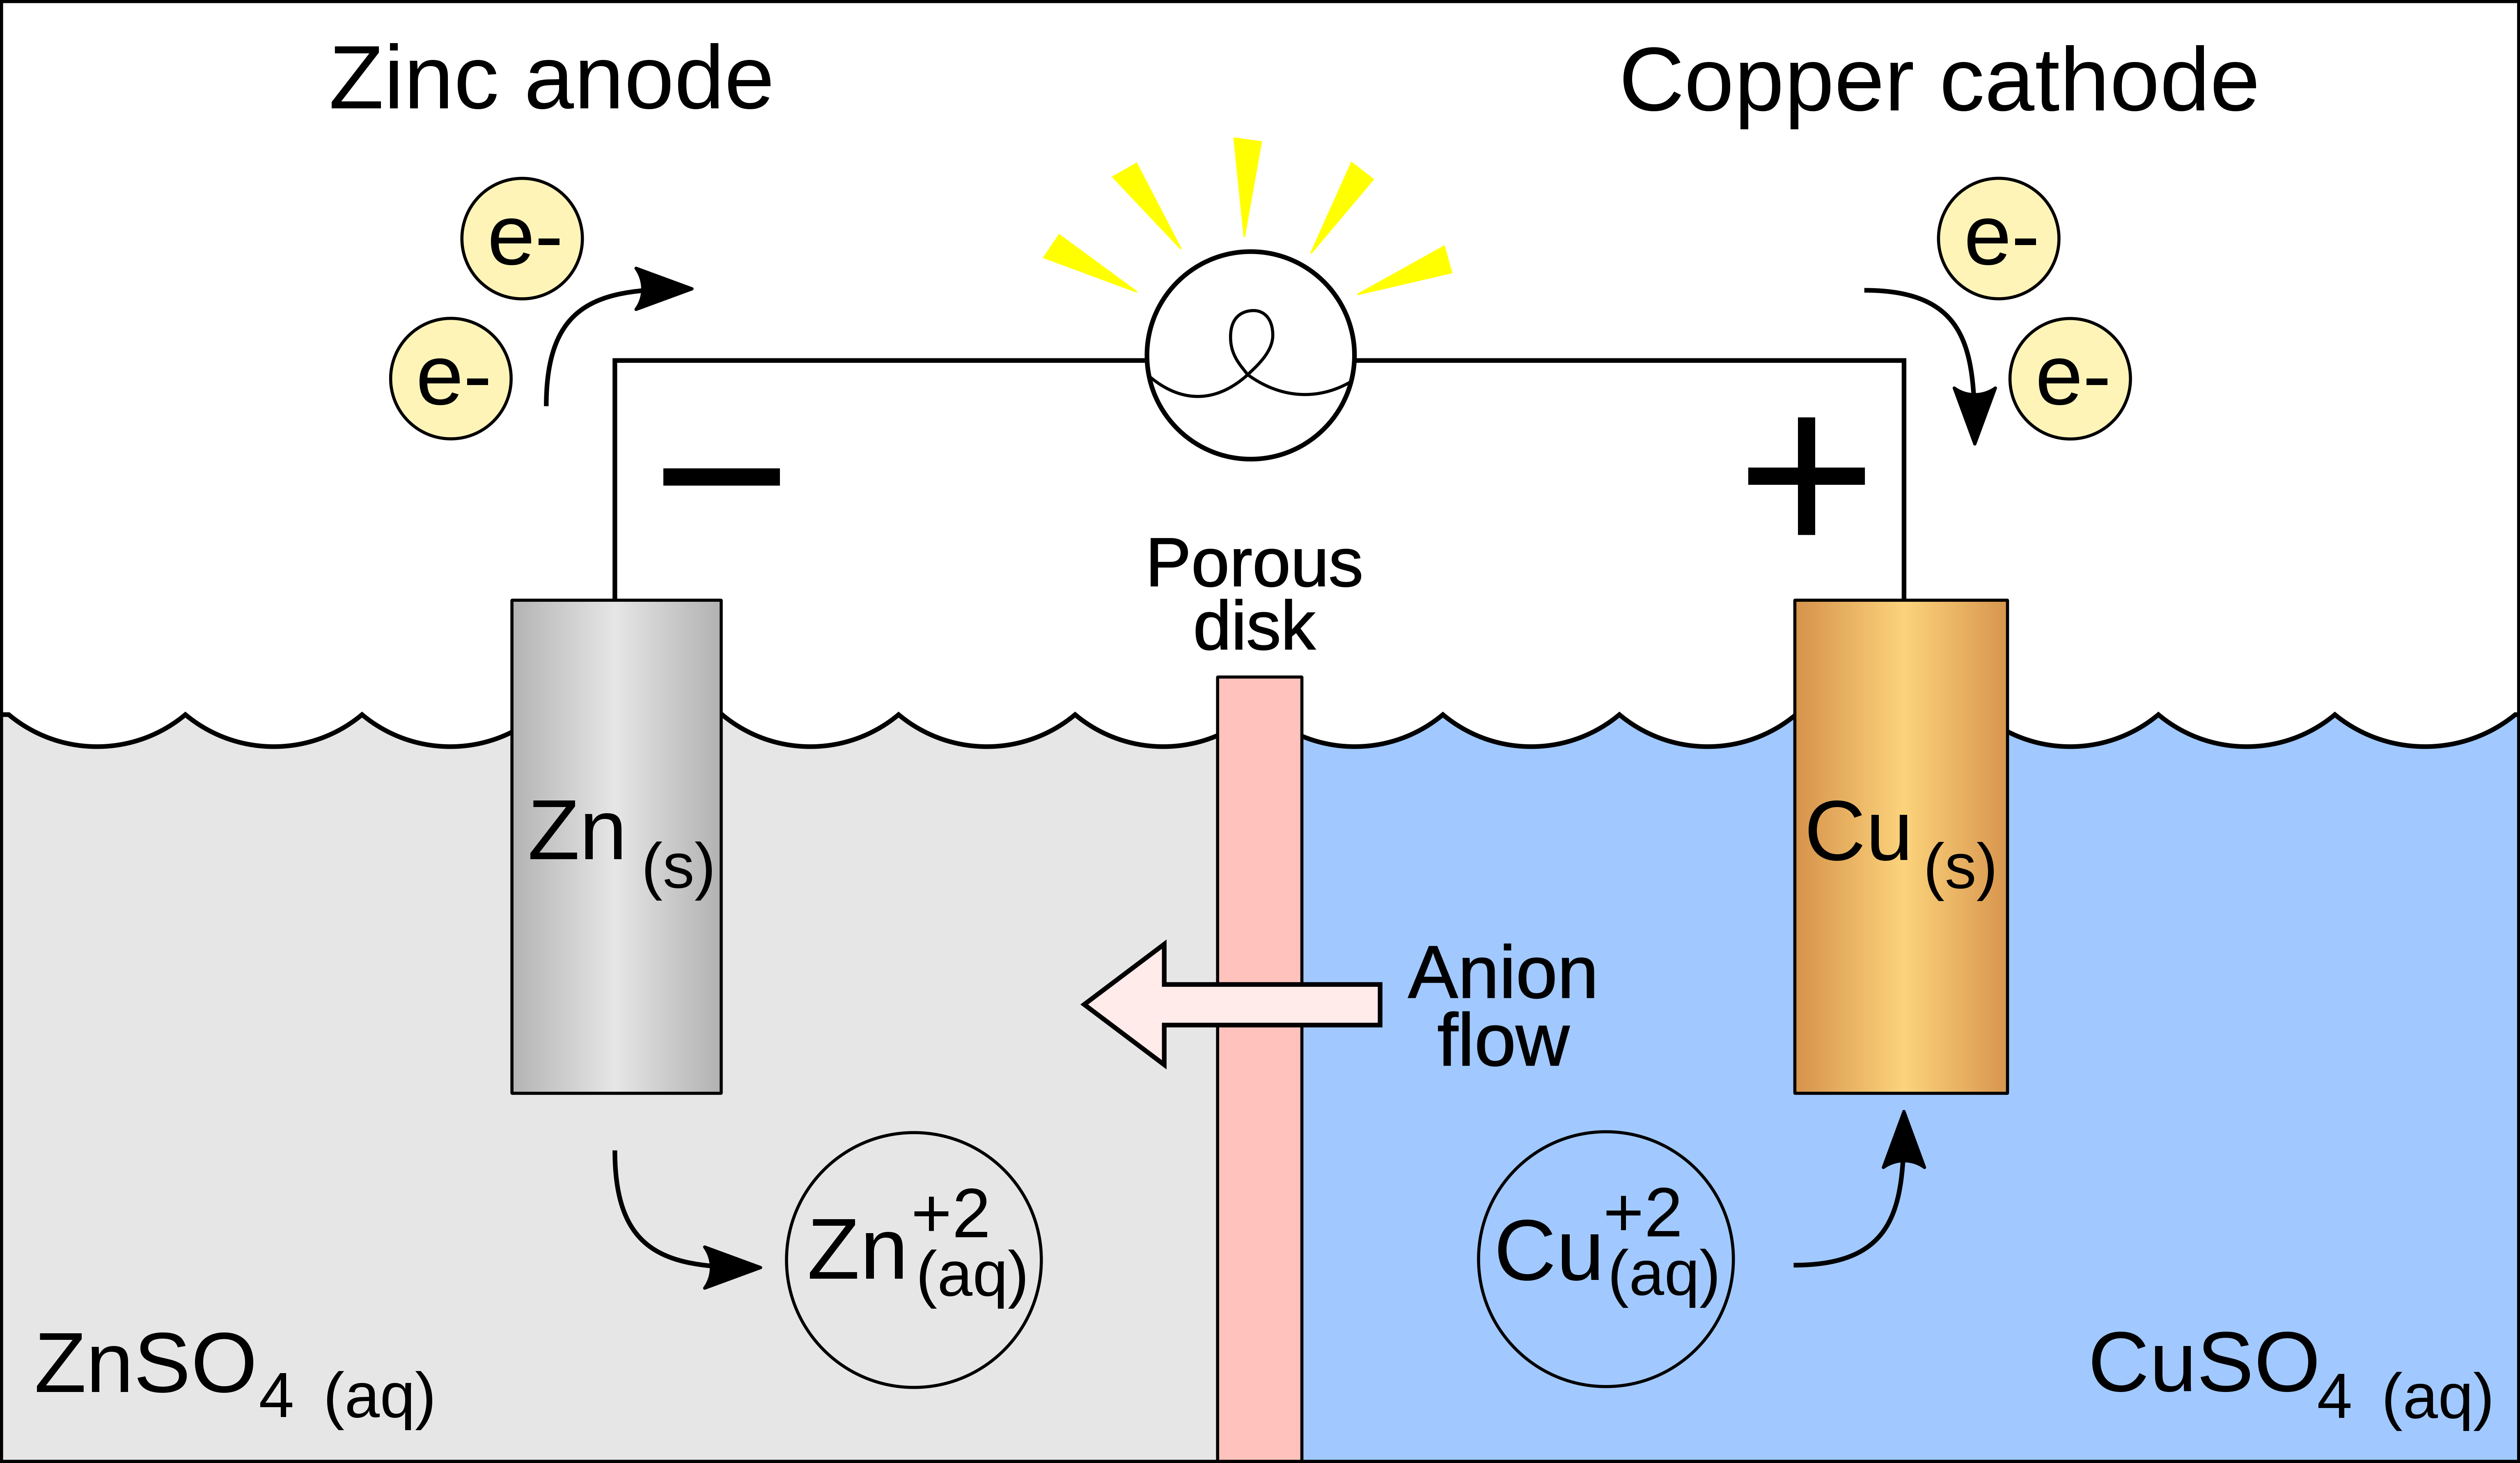
\includegraphics[width=.43\linewidth]{figs/Galvanic_cell.png}
	
		原电池和电解池中的电极命名通常采用下列原则：
		\begin{itemize}
			\item[\bullet] 按电势高低命名，电势高者为正极，低者为负极。
			\item[\bullet] 按电极反应类型命名，发生氧化反应者为阳极，发生还原反应者为阴极。
		\end{itemize}
		习惯上电解池用阴、阳极来命名，原电池用正、负极来命名。
		
		但有些场合下两种命名法都使用，在原电池中，负极是阳极，正极是阴极；在电解池中，正极是阳极，负极是阴极。    
	
	\end{frame}
	
	
	\begin{frame}
		\frametitle{法拉第定律}
	
		\large 电极上发生化学反应的物质的量与通过的电量成正比，通过相同的电量，不同物质发生反应的物质的量与其电荷数成反比，这就是法拉第定律（Faraday's law）
		\[
			q = \Delta n |Z|F
		\]
		$\Delta n$为电极上发生反应的物质的量(mol)；$q$为通过的电量(C)；$|Z|$为离子电荷数的绝对
	值；$F$为法拉第常量，\SI{96485}{C.mol^{-1}}。
		\begin{itemize}
			\item[\bullet] 法拉第定律是电化学上最早的定量的基本定律
			\item[\bullet] 该定律在任何温度、任何压力下均可以使用
		\end{itemize}
	
	\end{frame}
	
	
	\begin{frame}
		\frametitle{离子的电迁移}
	
		\large 在直流电场作用下，电解质溶液中的正、负离子分别向异电极方向移动，离子的这种运动称为\highlight{离子的电迁移}。
	
		离子迁移的速率除了与离子的本性（离子半径、所带电荷）以及溶液的黏度及温度有关外，还与电场的电势梯度$(\mathrm{d}E/\mathrm{d}l)$有关。离子迁移的动力来自电场，当电场稳定时，离子迁移速率$v$正比于电势梯度$(\mathrm{d}E/\mathrm{d}l)$，即
		\[
			v = U\frac{\mathrm{d}E}{\mathrm{d}l}
		\]
		式中，$U$称为\highlight{离子淌度}(ionic mobility)，表明电势梯度为单位数值时的离子迁移速率，单位是\si{m^2.V^{-1}.s^{-1}}
	
	\end{frame}
	
	
	\begin{frame}
		\frametitle{离子迁移数}
	
		\large 电解质溶液的导电是正、负离子向两极迁移电量叠加的结果，正、负离子同时承担着导电的任务，每种离子迁移的电量是不相同的。
	
		\highlight{离子迁移数}(transference number of ion)是指在一电解质溶液中各种离子的导电份额或导电百分数，用$t_\mathrm{B}$表示，即
		\[
			t_\mathrm{B}\equiv q_\mathrm{B}/q
		\]
		式中，$q_\mathrm{B}$为离子B传输的电量；$q$为通过溶液的总电量。
	
	\end{frame}
	
	
	\begin{frame}
		\frametitle{正、负离子的迁移数}
	
		对于只含有一种正离子和一种负离子的电解质溶液而言，正、负离子的迁移数分别为
		\[
			t_{+}=\frac{q_{+}}{q_{+}+q_{-}} \qquad t_{-}=\frac{q_{-}}{q_{+}+q_{-}}
		\]
		故
		\[
			t_{+}+t_{-}=1
		\]
		离子迁移数与离子淌度间的关系为
		\[
			t_{+}=\frac{U_{+}}{U_{+}+U_{-}} \qquad t_{-}=\frac{U_{-}}{U_{+}+U_{-}}
		\]
		由于离子淌度与电势梯度的强弱无关，可知离子迁移数也与电势梯度无关。
	
		影响离子迁移数的因素很多，如溶液浓度及种类、温度、离子半径、溶剂性质等。
	
	\end{frame}
	
	
	\begin{frame}
		\frametitle{}
	
	\begin{table}[]
		\caption{正离子的迁移数(298K)}
		\begin{tabular}{ccccc}
		\hline
		\rowcolor{maincolor!10} 
		\cellcolor{maincolor!10}                   & \multicolumn{4}{c}{\cellcolor{maincolor!10} 浓度/\si{(mol.dm^{-3})}} \\ \cline{2-5} 
		\rowcolor{maincolor!10} 
		\multirow{-2}{*}{\cellcolor{maincolor!10} \qquad 电解质 \qquad } &  ~~~~~~    0.01   ~~~~~~    &  ~~~~~~    0.05   ~~~~~~    &  ~~~~~~   0.10 ~~~~~~  &   ~~~~~~   0.20  ~~~~~~    \\ \hline
						HCl  &   0.825  &   0.829  &  0.831   &  0.834  \\
						NaCl  &  0.392   &  0.388   &  0.385   &  0.382  \\
						KCl   &     0.490      &     0.490      &     0.490      &    0.489      \\
						\ch{NH4Cl}   &     0.491      &     0.491      &      0.491     &      0.491    \\
						KBr   &     0.483      &     0.483      &     0.483      &     0.484     \\
						\ch{AgNO3}   &     0.465      &      0.466     &     0.468      &     -     \\
						\ch{KNO3}   &     0.508      &      0.509     &     0.510      &     0.512     \\
						\ch{1/2 CaCl2}   &     0.426      &     0.414      &      0.406     &      0.395    \\
						\ch{1/2 K2SO4}   &     0.483      &     0.487      &      0.489     &     0.491     \\ 
						   \hline
		\end{tabular}
		\end{table}
	
	\end{frame}

	
	\section{电导及其应用}


	\begin{frame}
		\frametitle{电导、电导率}
		\begin{enumerate}
			\item 电导
			
			导体的导电能力可用电导(conductance)$G$来表示，电导$G$为电阻$R$的倒数，$G=1/R$，单位是西门子(siemens)，符号为S。
			\item 电导率
			
			若导体具有均匀截面，其电导与截面积$A$成正比，与长度$l$成反比，即
			\[
				G = \kappa A/l
			\]
			式中$\kappa$为比例系数，称为电导率(conductivity)，单位为\si{S.m^{-1}}，它的物理意义是相距\SI{1}{m}的两个面积均为\SI{1}{m^2}的电极间溶液的电导，其值与电解质的种类、温度及浓度等因素有关。
		\end{enumerate}
	\end{frame}
	
	
	\begin{frame}
		\frametitle{摩尔电导率}
	
		摩尔电导率(molar conductlvity) $\Lambda_\mathrm{m}$表示在两个相距\SI{1}{m}的平行电极间，\SI{1}{mol}电解质溶液所具有的电导。由于电解质溶液的体积随浓度改变发生变化，$V=1/c$，故
		\[
			\Lambda_\mathrm{m} = \kappa/c
		\]
		式中：$\Lambda_\mathrm{m}$的单位为\si{S.m^2.mol^{-1}}，$c$的单位为\si{mol.m^{-3}}
		
		摩尔电导率$\Lambda_\mathrm{m}$有两种不同的表示法：
		\begin{enumerate}
			\item 以\SI{1}{mol}电荷的量为基本单元，本教材用此方法；
			\item 以\SI{1}{mol}电解质的量为基本单元。
		\end{enumerate}
		这两种表示方法对于1-1价型电解质是一致的，对于其他类型的电解质则不同。
	
		例如，用第一种方法，$\Lambda_\mathrm{m}(\ch{1/2 CuSO4}) = \SI{7.17e{-3}}{S.m^2.mol^{-1}}$
	
		用第二种方法，$\Lambda_\mathrm{m}(\ch{CuSO4}) = \SI{14.34e{-3}}{S.m^2.mol^{-1}}$
	
	\end{frame}
	
	
	\begin{frame}
		\frametitle{电导的测定}
	
		测定电解质溶液的电导，实际上是用韦斯顿(Weston)电桥测定电解质溶液的电阻。
		\begin{columns}[c]
			\column{8cm}
				
\includegraphics[width=\linewidth]{figs/fig5.2.png}
			\column{5.5cm}
				当电桥平衡时，
				\[
					\frac{R_x}{R_2}=\frac{R_3}{R_1}
				\]
				\[
					G=\frac{1}{R_x}=\frac{R_1}{R_2R_3}
				\]
		\end{columns}
		$R_x$为电导池，由两片固定在玻璃支架上的铂片组成。其距离与面积之比$l/A$称为电导池常数(cell constant)，可用已知电导率的标准溶液标定而得。
	\end{frame}
	
	
	\begin{frame}
		\frametitle{KCl溶液的电导率}
	\begin{table}[]
		\caption{KCl溶液的电导率}
		\begin{tabular}{ccccccc}
		\hline
		\rowcolor{maincolor!10} 
		\cellcolor{maincolor!10} & \multicolumn{6}{c}{\cellcolor{maincolor!10}电导率$\kappa$/\si{(S.m^{-1})}} \\ \cline{2-7} 
		\rowcolor{maincolor!10} 
		\multirow{-2}{*}{\cellcolor{maincolor!10} \si{c/(mol.dm^{-3})}} &   ~~273K~~    &   ~~278K~~    &   ~~283K~~    &    ~~288K~~   &    ~~293K~~   &    ~~298K~~  \\ \hline
			0.01    &   0.0766    &   0.0890    &   0.1020    &   0.1147    &   0.1278    &   0.1410   \\
			0.02    &   0.1521    &   0.1752    &   0.1994    &   0.2243    &   0.2501    &   0.2765   \\
			0.10    &   0.715    &   0.822    &    0.933   &    1.048   &   1.167    &   1.288   \\
			1.00    &   6.541    &   7.414    &   8.391    &   9.252    &   10.207    &   11.180   \\ \hline
		\end{tabular}
		\end{table}
	   
	\end{frame}
	
	
	\begin{frame}[t]
		\frametitle{}
	
		\begin{example}
			用一电导池在298K测得\SI{0.02}{mol.dm^{-3}}KCl溶液电阻为82.4$\Omega $，浓度为\SI{0.0050}{mol.dm^{-3}}的\ch{1/2 K2SO4}溶液电阻为326$\Omega $。试求(1)电导池常数$l/A$；（2）\SI{0.0050}{mol.dm^{-3}}\ch{1/2 K2SO4}溶液的电导率和摩尔电导率。
		\end{example}
		\pause
		(1)
		\[
		  l / A=\kappa / G=\kappa R=0.2765 \mathrm{~S} \cdot \mathrm{m}^{-1} \times 82.4 \Omega=22.8 \mathrm{~m}^{-1} 
		\]
		(2)
		\[
			\kappa^{\prime}=G \frac{l}{A}=\frac{1}{R} \frac{l}{A}=\frac{1}{326 \Omega} \times 22.8 \mathrm{~m}^{-1}=6.99 \times 10^{-2} \mathrm{~S} \cdot \mathrm{m}^{-1}
		\]
		\[
			\Lambda_{\mathrm{m}}=\kappa^{\prime} / c=\frac{6.99 \times 10^{-2} \mathrm{~S} \cdot \mathrm{m}^{-1}}{0.0050 \times 10^{3} \mathrm{~mol} \cdot \mathrm{m}^{-3}}=1.40 \times 10^{-2} \mathrm{~S} \cdot \mathrm{m}^{2} \cdot \mathrm{mol}^{-1}
		\]
	
	\end{frame}
	
	
	\begin{frame}
		\frametitle{强电解质溶液的电导率、摩尔电导率和浓度的关系}
	
		强电解质溶液的电导率随浓度增大而增加，当浓度达到一定值后，正负离子间相互作用增强，离子运动受到影响，电导率下降。
		
		弱电解质随浓度增大电离度减小，离子数目变化不大，其电导率随浓度的变化不明显。
		
		强电解质溶液的摩尔电导率随浓度减小而增大。溶液的浓度越低，离子间的距离越大，相互间作用力越小，含有lmol电荷的电解质溶液的导电能力越强。浓度很稀的强电解质溶液的摩尔电导率$\Lambda_{\mathrm{m}}$与溶液浓度的平方根$\sqrt{c}$之间有线性关系
		\[
			\Lambda_{\mathrm{m}}=\Lambda_{\mathrm{m}}^{\infty}(1-\beta \sqrt{c})    \]
		上式称为科尔劳乌施(Kohlrausch)公式。
	
	\end{frame}
	
	
	\begin{frame}
		\frametitle{强电解质溶液的电导率、摩尔电导率和浓度的关系}
		\begin{figure}[htb]
			\centering
			\begin{minipage}{0.48\linewidth}
			\centering
			
\includegraphics[width=.5\linewidth]{figs/fig5.3.png}
			\caption{电导率与浓度的关系}
			\end{minipage}\hfill
			\begin{minipage}{0.48\linewidth}
			\centering
			
\includegraphics[width=.7\linewidth]{figs/fig5.4.png}
			\caption{298K时一些电解质在水溶液中的摩尔电导率与浓度的关系}
			\end{minipage}
		\end{figure}
	\end{frame}
	
	
	\begin{frame}
		\frametitle{离子独立运动定律}
	
		科尔劳乌施经过研究提出了离子独立运动定律：在无限稀释溶液中电解质完全电离，并且离子间相互无影响。
	
		每种离子对溶液电导的贡献是独立的，电解质的无限稀释摩尔电导率$\Lambda_{\mathrm{m}}^\infty$是组成该电解质的正、负离子的无限稀释摩尔电导率的加和。
		
		1-1价型电解质
		\[
			\Lambda_{\mathrm{m}}^\infty = \Lambda_{\mathrm{m}^+}^\infty + \Lambda_{\mathrm{m}^-}^\infty
		\]
		$\mathrm{M}_{\nu_+}\mathrm{A}_{\nu_-}$价型电解质
		\[
			\Lambda_{\mathrm{m}}^\infty = {\nu_+}\Lambda_{\mathrm{m}^+}^\infty + {\nu_-}\Lambda_{\mathrm{m}^-}^\infty
		\]
		离子的无限稀释摩尔电导率取决于离子本性，在确定溶剂、温度等条件下是定值。利用离子独立运动定律，可以从已知离子的无限稀释摩尔电导率计算某一电解质的无限稀释摩尔电导率。
	
	\end{frame}
	
	
	\begin{frame}
		\frametitle{}
	
		\begin{table}[]
			\caption{某些离子的无限稀释摩尔电导率}
		\begin{tabular}{cccc}
		\hline
		\rowcolor{maincolor!10} 
		正离子 & $\Lambda_{\mathrm{m}}^\infty \times 10^{-4}/\si{S.m^2.mol^{-1}}$ & 负离子 & $\Lambda_{\mathrm{m}}^\infty \times 10^{-4}/\si{S.m^2.mol^{-1}}$ \\ \hline
		\ch{Ag+} & 61.9 & \ch{Br-} & 78.1 \\
		\ch{1/2 Ba^2+} & 63.9 & \ch{Cl-} & 76.35 \\
		\ch{1/2 Ca^2+} & 59.5 & \ch{F-} & 54.4 \\
		\ch{1/3 Fe^3+} & 68 & \ch{HCO3-} & 44.5 \\
		\red{\ch{H+}} & \red{349.82} & \ch{HSO4-} & 50 \\
		\ch{K+} & 73.5 & \ch{I-} & 76.8 \\
		\ch{Li+} & 38.69 & \ch{NO3-} & 71.4 \\    
		\ch{1/2 Mg^2+} & 53.06 & \red{\ch{OH-}} & \red{198.6} \\
		\ch{NH^4+} & 73.5 & \ch{1/3 PO4^3-} & 69.0 \\
		\ch{Na+} & 50.11 & \ch{Ac-} & 40.9 \\ \hline
		\end{tabular}
		\end{table}
	
	\end{frame}
	
	
	\begin{frame}[t]
		\frametitle{电导测定的应用}
	
		\begin{enumerate}
			\item[1.] \cbf{求弱电解质的电离度}
		\end{enumerate}
		弱电解质的$\Lambda_{\mathrm{m}}$和$\Lambda_{\mathrm{m}}^{\infty}$数值的大小分别反映溶液在一般情况下和无限稀释条件下的导电能力，它们之间的差别是因部分电离与全部电离产生的离子数目不同造成的，从而有
		\[
			\alpha = \frac{\Lambda_{\mathrm{m}}}{\Lambda_{\mathrm{m}}^{\infty}}
		\]
		式中$\alpha$即为该弱电解质在浓度$c$时的电离度。
	
		\begin{example}
			25℃时\SI{0.1000}{mol.dm^{-3}}的HAc溶液$\Lambda_{\mathrm{m}}=$\SI{5.201e4}{S.m^2.mol^{-1}}，求该HAc溶液的电离度。
		\end{example}
	
	\end{frame}
	
	
	\begin{frame}[t]
		\frametitle{电导测定的应用}
	
		\begin{enumerate}
			\item[2.] \cbf{检验水的纯度与计算水的离子积}
		\end{enumerate}
		在工农业生产、环境科学等众多领域，都需要水质检测，衡量水纯度的一个指标就是电导率。普通蒸馏水的电导率是\SI{1e{-3}}{S.m^{-1}}，重蒸馏水和去离子水的电导率均小于\SI{1e{-4}}{S.m^{-1}}。只要测定水的电导率就可以知道水中离子数量是否超标，纯度是否符合要求。水的离子积可以通过测定电导率来求。例如，25℃时纯水的密度为\SI{0.997e3}{kg.m^{-3}}，电导率$\kappa =$ \SI{5.5e{-6}}{S.m^{-1}}，则
			
		$\begin{aligned}
			c_{\mathrm{H}_{2} \mathrm{O}}&=\frac{0.997 \times 10^{3} \mathrm{~kg} \cdot \mathrm{m}^{-3}}{18.02 \times 10^{-3} \mathrm{~kg} \cdot \mathrm{mol}^{-1}}=55.3 \times 10^{3} \mathrm{~mol} \cdot \mathrm{m}^{-3}=55.3 \mathrm{~mol} \cdot \mathrm{dm}^{-3}\\
			\Lambda_{\mathrm{m}, \mathrm{H}_{2} \mathrm{O}}&=\frac{\kappa_{\mathrm{H}_{2} \mathrm{O}}}{c_{\mathrm{H}_{2} \mathrm{O}}}=\frac{5.5 \times 10^{-6} \mathrm{~S} \cdot \mathrm{m}^{-1}}{55.3 \times 10^{3} \mathrm{~mol}^{-3} \cdot \mathrm{m}^{-3}}\\
			&=0.99 \times 10^{-10} \mathrm{~S} \cdot \mathrm{m}^{2} \cdot \mathrm{mol}^{-1}
		\end{aligned}$
		
	
	\end{frame}
	
	
	\begin{frame}
		\frametitle{电导测定的应用}
	
		$\begin{aligned}
			\Lambda_{\mathrm{m}, \mathrm{H}_{2} \mathrm{O}}^{\infty}&=\Lambda_{\mathrm{m}, \mathrm{H^+}}^{\infty}+\Lambda_{\mathrm{m}, \mathrm{OH^-}}^{\infty}\\
			&=\left(3.498 \times 10^{-2}+1.986 \times 10^{-2}\right) \mathrm{S} \cdot \mathrm{m}^{2} \cdot \mathrm{mol}^{-1}\\
			&=5.484 \times 10^{-2} \mathrm{~S} \cdot \mathrm{m}^{2} \cdot \mathrm{mol}^{-1}\\
			\alpha&=\frac{\Lambda_{\mathrm{m}, \mathrm{H}_{2} \mathrm{O}}}{\Lambda_{\mathrm{m}, \mathrm{H}_{2} \mathrm{O}}^\infty}=\frac{0.99 \times 10^{-10} \mathrm{~S} \cdot \mathrm{m}^{2} \cdot \mathrm{mol}^{-1}}{5.484 \times 10^{-2} \mathrm{~S} \cdot \mathrm{m}^{2} \cdot \mathrm{mol}^{-1}}=1.8 \times 10^{-9} \qquad \text{水的电离度}\\
			c_{\mathrm{H}^{+}}&=c_{\mathrm{OH}^{-}}=\alpha c_{\mathrm{H}_{2} \mathrm{O}}\\
			&=1.8 \times 10^{-9} \times 55.3 \mathrm{~mol} \cdot \mathrm{dm}^{-3}\\
			&=1.0 \times 10^{-7} \mathrm{~mol} \cdot \mathrm{dm}^{-3}\\
			K_{\mathrm{w}}&=\frac{c_{\mathrm{H}^{+}}}{c^{\ominus}} \frac{c_{\mathrm{OH}}}{c^{\ominus}}=\left(1.0 \times 10^{-7}\right)^{2}=1.0 \times 10^{-14} \qquad \text{水的离子积}
			\end{aligned}$
	
	\end{frame}
	
	
	
	\begin{frame}[t]
		\frametitle{电导测定的应用}
	
		\begin{enumerate}
			\item[3.] \cbf{求难溶盐的溶解度和溶度积}
		\end{enumerate}
		某些难溶盐（如\ch{AgCl}，\ch{BaSO4}等）在水中溶解度极小，通常的化学分析方法难以直接测定，借助电导法则能很方便地测得。先测定难溶盐饱和溶液的电导率$\kappa $，实验测定的电解质溶液的电导率是溶液中所有电解质的电导率之和，从中减去高纯水的电导率即可得到难溶盐的电导率：
		\[
			\kappa_{\text{盐}} = \kappa_{\text{溶液}}  -\kappa_{\ch{H2O}}
		\]
		又根据摩尔电导率公式$\Lambda_{\mathrm{m}}=\frac{\kappa}{c}$，并且由于浓度很小可以近似认为难溶盐饱和溶液的$\Lambda_{\mathrm{m}} \approx \Lambda_{\mathrm{m}}^{\infty}$，因此
		\[
			c=\frac{\kappa_{\text{盐}}}{\Lambda_{\mathrm{m} \text{盐}}^{\infty}}
		\]
	
	\end{frame}
	
	
	\begin{frame}[t]
		\frametitle{电导测定的应用}
	
		\begin{enumerate}
			\item[4.] \cbf{电导滴定}
		\end{enumerate}
		\begin{minipage}{0.58\linewidth}
		利用滴定过程中体系电导的变化来判断滴定终点的方法称为电导滴定。电导滴定可用于酸碱中和反应、氧化-还原反应、沉淀反应等各类滴定反应。电导滴定不需要指示剂，故对于颜色较深或有混浊的溶液尤为有用，因为此时观察指示剂的变色较为困难。以中和滴定为例，图中a线表示强碱滴定强酸的曲线，b线为强碱滴定弱酸的曲线，虚线为滴定终点，两条线均有明显转折点，可以用来判断滴定终点。
		\end{minipage}\hfill
		\begin{minipage}{0.4\linewidth}
			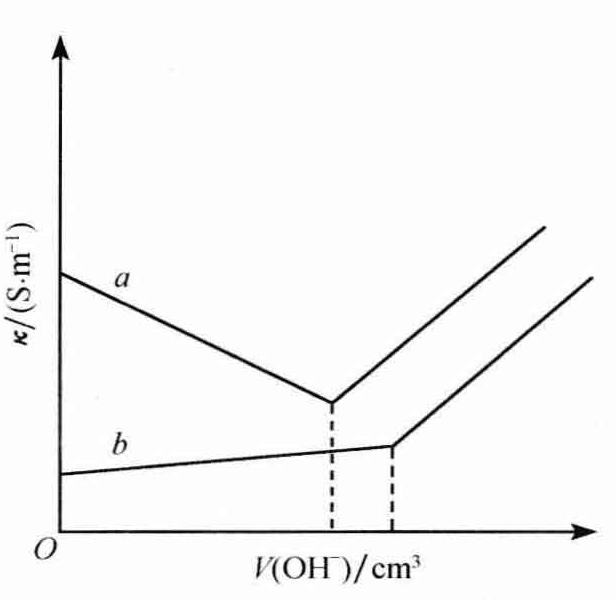
\includegraphics[width=\linewidth]{figs/fig5.6.png}
		\end{minipage}
	
	\end{frame}
	
	
	
	
	
	\begin{frame}[t]
		\frametitle{}
	
		\begin{example}
			298K时测得AgCl饱和溶液和高纯水的$\kappa $值分别为\SI{3.41e{-4}}{S.m^{-1}}和\SI{1.60e{-4}}{S.m^{-1}}，计算该温度下AgCl的溶解度和溶度积。
		\end{example}
		\pause
		$\begin{aligned}
			\kappa_{\mathrm{AgCl}}&=\kappa_{\mathrm{AgCl} \text {溶液}}-\kappa_{\mathrm{H}_{2} \mathrm{O}}=(3.41-1.60) \times 10^{-4}=1.81 \times 10^{-4} \mathrm{~S}\cdot \mathrm{m}^{-1}\\
			\Lambda_{\mathrm{m}}^{\infty}(\mathrm{AgCl})&=\Lambda_{\mathrm{m}}^{\infty}\left(\mathrm{Ag}^{+}\right)+\Lambda_{\mathrm{m}}^{\infty}\left(\mathrm{Cl}^{-}\right)=1.38 \times 10^{-2} \mathrm{~S} \cdot \mathrm{m}^{2} \cdot \mathrm{mol}^{-1}\\
			c&=\frac{\kappa}{\Lambda_{\mathrm{m}}^{\infty}}=\frac{1.81 \times 10^{-4} \mathrm{~S} \cdot \mathrm{m}^{-1}}{1.38 \times 10^{-2} \mathrm{~S} \cdot \mathrm{m}^{2} \cdot \mathrm{mol}^{-1}}=1.31 \times 10^{-5} \mathrm{~mol} \cdot \mathrm{dm}^{-3}\\
			K_{\mathrm{sp}}&=\frac{c_{\mathrm{Ag}}^+}{c^{\ominus}} \frac{c_{\mathrm{Cl}}^{-}}{c^{\ominus}}=\left(1.31 \times 10^{-5}\right)^{2}=1.72 \times 10^{-10}\\
			S&=\left(143.4 \times 1.31 \times 10^{-5}\right) \mathrm{g} \cdot \mathrm{dm}^{-3}=1.88 \times 10^{-3} \mathrm{~g}\cdot{\mathrm{dm}^{-3}}
		\end{aligned}$
	
	\end{frame}


	\section{强电解质溶液的活度及活度系数}


	\begin{frame}
		\frametitle{电解质溶液的化学势}
	
		溶液中溶质的活度为$a_\mathrm{B}=\gamma_\mathrm{B}b_\mathrm{B}/b^\ominus$，其化学势为$\mu_\mathrm{B}=\mu_\mathrm{B}^\ominus + RT \ln a_\mathrm{B}$。
		
		对于电解质溶液来说情况更为复杂。在电解质溶液中独立运动的粒子是离子，因此以正、负离子的活度来表示相对应离子的化学势。
		\[
			\mu_\mathrm{+}=\mu_\mathrm{+}^\ominus + RT \ln a_\mathrm{+} \qquad \mu_\mathrm{-}=\mu_\mathrm{-}^\ominus + RT \ln a_\mathrm{-}
		\]
		
		其中正、负离子的活度分别为
		\[
			a_\mathrm{+}=\gamma_\mathrm{+}b_\mathrm{+}/b^\ominus \qquad a_\mathrm{-}=\gamma_\mathrm{-}b_\mathrm{-}/b^\ominus
		\]
		任意强电解质$\mathrm{M}_{\nu_+}\mathrm{A}_{\nu_-}$的化学势与正、负离子的化学势的关系为
		$\begin{aligned}
			\mu_{\mathrm{M}_{\nu_{+}} A_{\nu_-}} &=\nu_+ \mu_{+}+\nu_-\mu_{-}=(\nu_{+} \mu_{+}^{\ominus}+\nu_{-} \mu_{-}^{\ominus})+R T \ln (a_{+}^{\nu_{+}} a_{-}^{\nu_-}) \\
			&=\mu_{\mathrm{M}_{\nu_{+}} \mathrm{A}_{\nu_-}}^{\ominus}+R T \ln a_{\mathrm{M}_{\nu+} \mathrm{A}_{\nu_-}}
			\end{aligned}$
	
	\end{frame}
	
	
	\begin{frame}
		\frametitle{活度和活度系数}
	
		电解质活度与其正、负离子活度的关系式
		\[
			a_{\mathrm{M}_{\nu_{+}} A_{\nu_-}}=a_{+}^{\nu_{+}} a_{-}^{\nu_-}
		\]
		由于溶液中正、负离子总是同时存在的，因此用实验方法难以测得单种离子的活度。通常用可以测定的物理量-离子平均活度$a_\pm$来代替$a_+$和$a^-$
		
		$a_+$的定义为
		\[
			a_{\pm} \stackrel{\text { def }}{=}(a_{+}^{\nu_{+}} a_{-}^{\nu_-})^{1 / \nu}
		\]
		平均活度系数$\gamma_\pm$和平均质量摩尔浓度$b_\pm$的定义为
		\[
			\gamma_{\pm}=(\gamma_{+}^{\nu_{+}} \gamma_{-}^{\nu_-})^{1 / \nu} 
		\]
		\[
			b_{\pm}=(b_{+}^{\nu_{+}} b_{-}^{\nu_-})^{1 / \nu} 
		\]
		式中，$\nu = \nu_+ + \nu_-$
	
	\end{frame}
	
	
	\begin{frame}
		\frametitle{活度和活度系数}
	
		电解质活度与离子平均活度间的关系为
		\[
			a_{\mathrm{M}_{\nu_{+}} \mathrm{A}_{\nu_-}}=a_{+}^{\nu_{+}} a_{-}^{\nu_-}=a_{\pm}^{\nu}
		\]
		平均活度与平均活度系数、平均质量摩尔浓度间的关系为
		\[
			a_{\pm}=\gamma_{\pm} b_{\pm} / b^{\ominus}
		\]
		$\gamma_{\pm}$和$b_{\pm}$虽有相似的定义式，但不能就此认为$b_{\mathrm{M}_{\nu_{+}} \mathrm{A}_{\nu_-}}=b_{\pm}^\nu$，事实上
		\[
			b_+=\nu_+b_\mathrm{B} \qquad b_-=\nu_-b_\mathrm{B}
		\]
		\[
			b_{\pm}^{\nu}=(\nu_{+} b_{\mathrm{B}})^{\nu_{+}}(\nu_{-} b_{\mathrm{B}})^{\nu_-}=(\nu_{+}^{\nu_{+}} \nu_{-}^{\nu-}) b_{\mathrm{B}}^{\nu}
		\]
		\[
			b_{\pm}=(\nu_{+}^{\nu_{+}} \nu_{-}^{\nu-})^{1 / \nu} b_{\mathrm{B}}
		\]
	
	\end{frame}
	
	
	\begin{frame}[t]
		\frametitle{}
	
		\begin{example}
			现有\SI{0.1}{mol.kg^{-1}}\ch{La2(SO4)3}溶液，求其平均浓度$b_{\pm}$。
		\end{example}
		\pause
		\[
			\nu_{+}=2 \qquad \nu_{-}=3        
		\]
		\[
			\nu=5
		\]
		\[
			b_\mathrm{B}=\SI{0.1}{mol.kg^{-1}}
		\]
		\[
			b_{\pm}=(\nu_+^{\nu^+} \nu_-^{\nu_-})^{1 / \nu} b_{\mathrm{B}}=(2^{2} \times 3^{3})^{1 / 5} \times 0.1 \mathrm{~mol} \cdot \mathrm{kg}^{-1}=0.3 \mathrm{~mol} \cdot \mathrm{kg}^{-1}
		\]
	
	\end{frame}
	
	
	\begin{frame}
		\frametitle{}
	
	\begin{table}[]
		\caption{一些电解质在水溶液中的平均活度系数$\gamma_\pm$\ (298K)}
		\label{tab:my-table}
		\begin{tabular}{cccccccccc}
		\hline
		\rowcolor{maincolor!10} 
		\cellcolor{maincolor!10}                   & \multicolumn{9}{c}{\cellcolor{maincolor!10}浓度/(\si{mol.dm^{-3}})} \\ \cline{2-10} 
		\rowcolor{maincolor!10} 
		\multirow{-2}{*}{\cellcolor{maincolor!10}电解质} &   0.001  &  0.002   &  0.005  &  0.01  &  0.05  &  0.1  &  0.5  &  1.0  &  3.0  \\ \hline
			HCl   &  0.966   &   0.952  &  0.928  &  0.904  &  0.830  &  0.798  &  0.768  &  0.809  &  1.31  \\
			KOH   &  -   &   -  &  0.90  &  0.818  &  0.766  &  0.690  &  0.688  &  0.678  &  -  \\
			KCl   &  0.965   &  0.952   &  0.923  &  0.901  &  0.815  &  0.769  &  0.651  &  0.606  &  0.572  \\
			NaCl   &   0.965  &   0.952  &  0.927  &  0.912  &  0.819  &  0.778  &  0.682  &  0.658  &   0.719 \\
			\ch{H2SO4}   &   0.830  &   0.757  &  0.608  &  0.544  &  0.340  &  0.255  &  0.154  &  0.100  &  0.142  \\
			\ch{Na2SO4}   &   0.887  &   0.847  &  0.778  &  0.714  &  0.536  &  0.453  &  0.270  &  0.204  &  -  \\
			\ch{ZnSO4}    &   0.700  &   0.508  &  0.477  &  0.387  &  0.202  &  0.150  &  0.063  &  0.044  &  0.041  \\
			\ch{ZnCl2}    &   0.88  &   0.84  &  0.789  &  0.731  &  0.578  &  0.515  &  0.429  &  0.337  &  -  \\ \hline
		\end{tabular}
		\end{table}
	
	\end{frame}
	
	
	
	\begin{frame}
		\frametitle{影响离子平均活度系数的因素}
	
		\begin{enumerate}
			\item 稀溶液离子平均活度系数的值随浓度降低而增大，在无限稀释时达到1。
			\item 溶液浓度高时，随浓度增大离子平均活度系数增大，甚至大于1。
			\item 离子电荷数对$\gamma_{\pm}$影响较大。
			\item 溶液中其他电解质对$\gamma_{\pm}$也会产生影响，说明与溶液整体电解质含量有关。
		\end{enumerate}
		综上所述，在一定温度下，离子平均活度系数$\gamma_{\pm}$与溶液整体的离子浓度以及所含离子的电荷数有关。路易斯于1921年提出了离子强度$I$的概念
		\[
			I \equiv \frac{1}{2}\sum_\mathrm{B}{b_\mathrm{B}Z_\mathrm{B}^2}
		\]
		\[
			\lg \gamma_{\pm} = -A'\sqrt{I/b^\ominus}
		\]
		$Z_\mathrm{B}$为离子B的电荷数，$A'$为常数，与温度、溶剂种类有关。
	
	\end{frame}
	
	
\end{document}